\section{Einleitung}

Die Einleitung \cite{iptables}

\subsection{Begriffsdefinitionen}

Masquarading? Hier oder im Konfig Kapitel?

Connection Tracking? Hier oder im Konfig Kapitel?

\paragraph{DMZ}
Wenn als Computernetzwerkbegriff verstanden ist die
\emph{demilitarisierte Zone} ein Bereich in dem Dienste einer Firma die nach Außen,
also z.B. das Internet oder Extranet, angeboten werden. Diese Dienste sollen
vom eigentelichen LAN in einem abgeschotteten Bereich laufen, so dass
beispielsweise die Mitarbeiterrechner sicher sind.


\section{Versuchsaufbau}

Ziel ist es das Firmen-LAN sowie die zugehörige DMZ durch die
{\tt iptables} Linux-Firewall abzusichern.

\begin{figure}[h!]
  \centering
    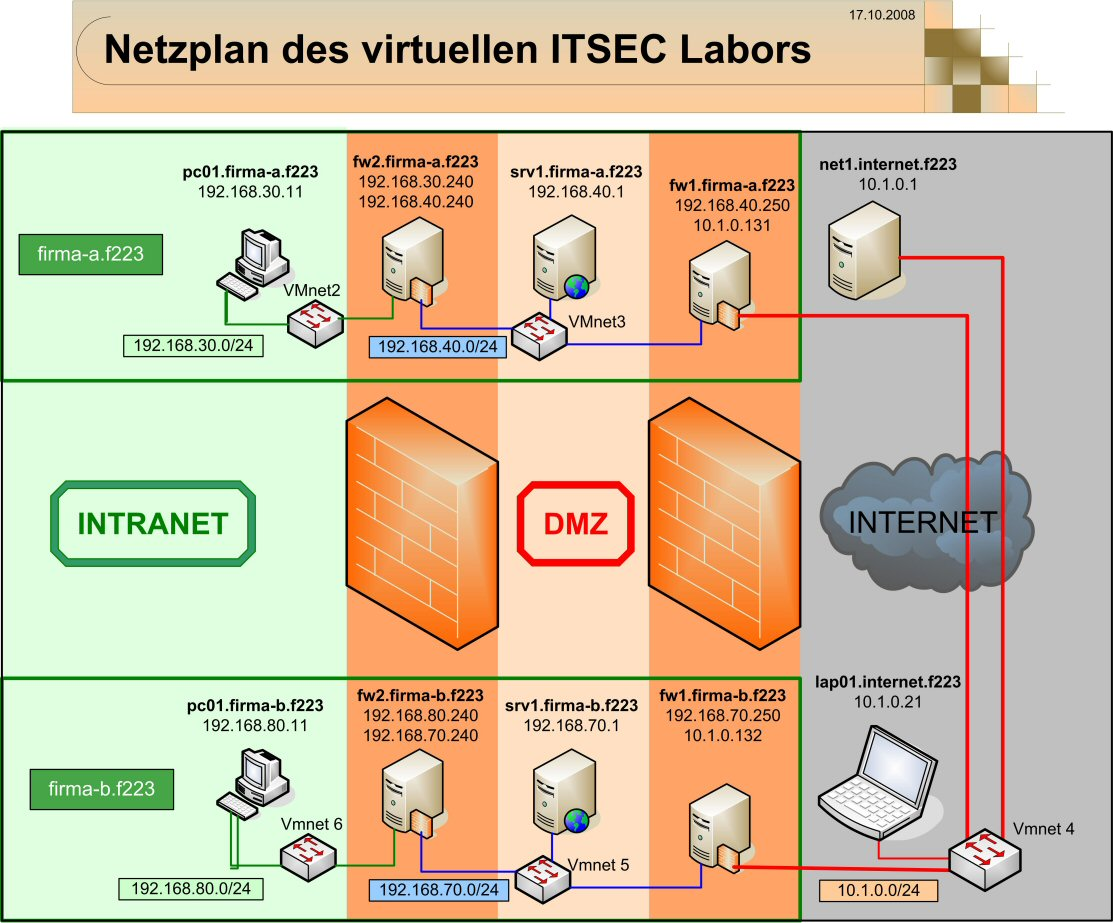
\includegraphics[width=0.9\textwidth]{figures/Netzplan.jpg}
  \caption{Netzplan des Versuchsaufbaus.\cite{labor}}
  \label{fig.netzplan}
\end{figure}

Dazu sind im Versuchsaufbau für jeden der in Abbildung 
\ref{fig.netzplan} abgebildeten Rechner
eine virtuelle Maschine bereitgestellt---dies ermöglicht leichteres
Testen.

Wir haben uns dazu entschieden, das Netzwerk der \emph{Firma A} aufzubauen.
Firma B bleibt unangetastet, und ist somit vollständig vorkonfiguriert,
was ein leichteres Testen ermöglicht.\cite{labor}


\section{Linux Konfiguration}

Zunächst müssen zwei Debian 6.0 Maschinen,
mit der minimalen Installation, eingerichtet werden.
Diese repräsentieren die Firewallmaschinen {\tt fw1} und {\tt fw2} aus
Abbildung \ref{fig.netzplan}.
Es wurde noch weitere Software installiert,
beschrieben in Kapitel \ref{sec.software}.
Die genaue Netzwerkadapterkonfiguration ist in Kapitel \ref{sec.netzwerk}

\subsection{Software}\label{sec.software}

Zusätzliche Software wurde via {\tt apt-get}, Debians Paketmanager,
installiert.

\begin{itemize}
    \item iptables
    \item iptstate---IPTables State Top.
    \item resolvconf---Nameserver information handler.
\end{itemize}


\subsection{Netzwerkadapter}\label{sec.netzwerk}

Die Netzweradapter wurden gemäß der in Abbildung \ref{fig.netzplan}
gezeigten IP-Adressen konfiguriert.
Die Konfigurationsdatei dazu liegt in {\tt /etc/network/interfaces}.

\subsubsection{Extranet $\Longleftrightarrow$ DMZ}

Ist Firewall {\tt fw1} die zwischen Extranet $\Longleftrightarrow$ DMZ sitzt.

\paragraph{eth0} Verbindung zur DMZ.

\begin{lstlisting}[label=lst:dmz:eth0,caption={Netzwerkadapter eth0 Konfiguration.}]
allow-hotplug eth0
iface eth0 inet static
    address 192.168.40.250
    netmask 255.255.255.0
    broadcast 192.168.40.255
    dns-nameservers 192.168.40.1
    dns-search firma-a.f223
\end{lstlisting}

\paragraph{eth1} Verbindung zum Extranet bzw. Internet.

\begin{lstlisting}[label=lst:extranet:eth1,caption={Netzwerkadapter eth1 Konfiguration.}]
allow-hotplug eth1
iface eth1 inet static
    address 10.1.0.131
    netmask 255.255.255.0
    broadcast 10.1.0.0
\end{lstlisting}


\subsubsection{DMZ $\Longleftrightarrow$ Intranet}

Ist Firewall {\tt fw2} die zwischen DMZ $\Longleftrightarrow$ Intranet sitzt.

\paragraph{eth0} Verbindung zum Intranet.

\begin{lstlisting}[label=lst:dmz:eth0,caption={Netzwerkadapter eth0 Konfiguration.}]
allow-hotplug eth0
iface eth0 inet static
    address 192.168.30.240
    netmask 255.255.255.0
    network 192.168.30.0
    broadcast 192.168.30.255
    dns-search firma-a.f223
\end{lstlisting}

\paragraph{eth1} Verbindung zur DMZ.

\begin{lstlisting}[label=lst:extranet:eth1,caption={Netzwerkadapter eth1 Konfiguration.}]
allow-hotplug eth1
iface eth1 inet static
    address 192.168.40.240
    netmask 255.255.255.0
    network 192.168.40.0
    broadcast 192.168.40.255
    dns-nameservers 192.168.40.1
\end{lstlisting}


\subsection{Nützliches}

\paragraph{Einfacher Dateitransfer}

Empfänger:
{\tt fw2\# netcat -l -p 8080 > firewall-internal.sh}

Sender:
{\tt fw1\# cat firewall-external.sh | netcat 192.168.40.240 8080}


\subsection{Bootskript}

Debian verwendet das sogenannte \emph{Init Script LSB}\footnote{
\url{http://wiki.debian.org/LSBInitScripts}}, welches Unterstützung
für \emph{dependency based boot sequencing}\footnote{
\url{http://wiki.debian.org/LSBInitScripts/DependencyBasedBoot}
} bietet. Das bedeutet, dass
die Programme die beim Aufstarten des Betriebssystems in einer idealen
Reihenfolge angeordnet werden, so dass es auch keine unangenehme Effekte
durch Abhängigkeiten der Programme untereinander entstehen.

Diese Bootskripte werden in {\tt /etc/init.d/} als Konfigurationsdateien
abgelegt und beginnen mit wohldefinierten Kopfzeilen, wie in Listing
\ref{lst:lsb-header} gezeigt. In diesen Zeilen können die Abhängigkeiten
konfiguriert werden.

\begin{lstlisting}[label=lst:lsb-header,caption={Init Script LSB: Kopfzeilen.}]
### BEGIN INIT INFO
# Provides:          scriptname
# Required-Start:    $remote_fs $syslog
# Required-Stop:     $remote_fs $syslog
# Default-Start:     2 3 4 5
# Default-Stop:      0 1 6
# Short-Description: Start daemon at boot time
# Description:       Enable service provided by daemon.
### END INIT INFO
\end{lstlisting}

Wenn \emph{dependency-based booting} aktiviert ist, wird ein Daemon mit seinem
Startupskript aus {\tt /etc/init.d/} mit {\tt insserv}\footnote{
\emph{Vor} Debian 6.0 wird {\tt update-rc.d} verwendet.
} gestartet:

\begin{verbatim}
insserv mydaemon_script
\end{verbatim}

Nach den Kopfzeilen kommt das eigentliche Skript, welches z.B. mittels
{\tt iptables} die Firewall konfiguriert, aber auch beliebige andere Programme
und Dienste können somit gestartet werden.

\begin{lstlisting}[label=lst:lsb-script,caption={Init Script LSB: Eigentliches Skript.}]
case "$1" in
    start)
        # Startup stuff
        echo "Daemon started."
        ;;
    stop)
        # Shutdown this service
        echo "Daemon stopped."
        ;;
    restart)
        # Restart this service
        echo "Daemon restarted."
        ;;
    *)
        # The default case
        echo "Usage $0 {start|stop|restart}"
        ;;
esac
\end{lstlisting}



\section{Firewall Konfiguration}

\subsection{Extranet $\Longleftrightarrow$ DMZ}

Ist Firewall {\tt fw1} die zwischen Extranet $\Longleftrightarrow$ DMZ sitzt.


\subsubsection{Initialisierung}

\paragraph{Anforderung} Grundlegende Initialisierung der Firewall, d.h.
sie nimmt alle Pakete an. Zugriff auf Rechner innerhalb der DMZ ist ohne
weitere Regeln jedoch \emph{nicht} möglich, also \emph{keine} Weiterreichung von
Pakten.

\paragraph{Konfiguration} Diese Konfigurationsdatei aus Listing \ref{lst:init}
befindet sich in {\tt /etc/init.d/firewall-external.sh}.
Das Skript wird mit dem Befehl {\tt chmod u+x firewall-external.sh}
ausführbar gemacht. Mit {\tt insserv firewall-external.sh}
wird das Skript auch beim Aufstarten der Maschine automatisch ausgeführt,
und damit die Firewall aktiviert.

\begin{lstlisting}[label=lst:init,caption={Basis Firewall Bootskript.}]
#!/bin/sh
### BEGIN INIT INFO
# Provides:          external firewall
# Required-Start:    $local_fs $remote_fs $syslog $network
# Required-Stop:     $local_fs $remote_fs $syslog $network
# Default-Start:     2 3 4 5
# Default-Stop:      0 1 6
# Short-Description: External firewall
# Description:       External firewall (sh, mb)
### END INIT INFO

case "$1" in
    start)
        # clear
        iptables -F
        iptables -t nat -F
        iptables -t mangle -F
        iptables -x

        # defaults
        iptables -P INPUT   ACCEPT
        iptables -P OUTPUT  ACCEPT
        iptables -P FORWARD ACCEPT

        # loopback
        iptables -A INPUT  -i lo -j ACCEPT
        iptables -A OUTPUT -o lo -j ACCEPT

        # stateful rules (after that, only need to allow NEW connections)
        iptables -A INPUT   -m conntrack --ctstate ESTABLISHED,RELATED -j ACCEPT
        iptables -A OUTPUT  -m conntrack --ctstate ESTABLISHED,RELATED -j ACCEPT
        iptables -A FORWARD -m conntrack --ctstate ESTABLISHED,RELATED -j ACCEPT

        # drop invalid state packets
        iptables -A INPUT   -m conntrack --ctstate INVALID -j DROP
        iptables -A OUTPUT  -m conntrack --ctstate INVALID -j DROP
        iptables -A FORWARD -m conntrack --ctstate INVALID -j DROP

        echo "Firewall started."
        ;;

    stop)
        iptables -F
        iptables -P INPUT  ACCEPT
        iptables -P OUTPUT ACCEPT

        echo "Firewall disabled."
        ;;

    restart)
        $0 stop
        sleep 1
        $0 start
        ;;

    *)
        echo "Usage $0 {start|stop|restart}"
        ;;

esac
\end{lstlisting}
%\lstinputlisting[language=Python, firstline=37, lastline=45]{source_filename.py}

\paragraph{Test} Über die virtuelle Maschine {\tt lap1.internet.f223} wird
via {\tt ping} getestet, ob eine Verbindung zwischen {\tt lap1} und {\tt fw1}
möglich ist.


\subsubsection{Weiterleitung auf Server}

\paragraph{Anforderung} Pakete sollten vom Extranet über die Firewall an
den Web- und Mailserver {\tt srv1}, weitergeleitet werden.
Es laufen HTTP auf Port 80, HTTPS auf Port 443 und SMTP auf Port 25.

\paragraph{Konfiguration} Das Listing \ref{lst:webserver} ist das Skript
aus Listing \ref{lst:init}, entsprechend erweitert.
Es wird die Option {\tt DNAT} gewählt, womit das Ziel umgebogen wird.
Die Firewall sieht von Außen nun aus wie der jeweilige Server.

\begin{lstlisting}[label=lst:webserver,caption={Web- und Mailserver Forwarding.}]
#!/bin/sh
### BEGIN INIT INFO
# Provides:          external firewall
# Required-Start:    $local_fs $remote_fs $syslog $network
# Required-Stop:     $local_fs $remote_fs $syslog $network
# Default-Start:     2 3 4 5
# Default-Stop:      0 1 6
# Short-Description: External firewall
# Description:       External firewall (sh, mb)
### END INIT INFO

SRV_IP=192.168.40.1
FW2_IP=192.168.40.240
DMZ_IP=192.168.40.250
EXT_IP=10.1.0.131

forwardToSrv()
{
    PORT=$1
    iptables -t nat -A PREROUTING -p tcp -i eth1 --dport $PORT -j DNAT --to $SRV_IP
}

case "$1" in
    start)
        # clear
        iptables -F
        iptables -t nat -F
        iptables -t mangle -F
        iptables -x

        # defaults
        iptables -P INPUT   ACCEPT
        iptables -P OUTPUT  ACCEPT
        iptables -P FORWARD ACCEPT

        # enable Forwarding
        echo "1" > /proc/sys/net/ipv4/ip_forward

        # loopback
        iptables -A INPUT  -i lo -j ACCEPT
        iptables -A OUTPUT -o lo -j ACCEPT

        # stateful rules (after that, only need to allow NEW connections)
        iptables -A INPUT   -m conntrack --ctstate ESTABLISHED,RELATED -j ACCEPT
        iptables -A OUTPUT  -m conntrack --ctstate ESTABLISHED,RELATED -j ACCEPT
        iptables -A FORWARD -m conntrack --ctstate ESTABLISHED,RELATED -j ACCEPT

        # drop invalid state packets
        iptables -A INPUT   -m conntrack --ctstate INVALID -j DROP
        iptables -A OUTPUT  -m conntrack --ctstate INVALID -j DROP
        iptables -A FORWARD -m conntrack --ctstate INVALID -j DROP

        # port Forwarding from extranet
        forwardToSrv  25  # smtp
        forwardToSrv  80  # http
        forwardToSrv 443  # https

        echo "Firewall started."
        ;;

    stop)
        iptables -F
        iptables -P INPUT  ACCEPT
        iptables -P OUTPUT ACCEPT

        echo "Firewall disabled."
        ;;

    restart)
        $0 stop
        sleep 1
        $0 start
        ;;

    *)
        echo "Usage $0 {start|stop|restart}"
        ;;

esac
\end{lstlisting}

\paragraph{Test} Über den Browser des Client-Rechner {\tt lap1},
der sich im Extranet befindet.


\subsubsection{Masquerading}

\paragraph{Anforderung}
Dabei soll {\tt pc01} nach außen hin wirken wie wenn die Anfrage von
{\tt fw1} kommt.

Hier wird also der Rückkanal von {\tt fw1} zu {\tt pc01} gebildet.

\paragraph{Konfiguration}

\begin{lstlisting}[label=lst:masq,caption={Masquerading.}]
#!/bin/sh
### BEGIN INIT INFO
# Provides:          external firewall
# Required-Start:    $local_fs $remote_fs $syslog $network
# Required-Stop:     $local_fs $remote_fs $syslog $network
# Default-Start:     2 3 4 5
# Default-Stop:      0 1 6
# Short-Description: External firewall
# Description:       External firewall (sh, mb)
### END INIT INFO

SRV_IP=192.168.40.1
FW2_IP=192.168.40.240
DMZ_IP=192.168.40.250
DMZ_DEV="eth0"
EXT_IP=10.1.0.131
EXT_DEV="eth1"

forwardToSrv()
{
    PORT=$1
    iptables -t nat -A PREROUTING -p tcp -i $EXT_DEV --dport $PORT -j DNAT --to $SRV_IP
}

case "$1" in
    start)
        # clear
        iptables -F
        iptables -t nat -F
        iptables -t mangle -F
        iptables -x

        # defaults
        iptables -P INPUT   ACCEPT
        iptables -P OUTPUT  ACCEPT
        iptables -P FORWARD ACCEPT

        # enable Forwarding
        echo "1" > /proc/sys/net/ipv4/ip_forward

        # fw2 as gateway to lan
        route add -net 192.168.30.0 netmask 255.255.255.0 gw $FW2_IP

        # loopback
        iptables -A INPUT  -i lo -j ACCEPT
        iptables -A OUTPUT -o lo -j ACCEPT

        # stateful rules (after that, only need to allow NEW connections)
        iptables -A INPUT   -m conntrack --ctstate ESTABLISHED,RELATED -j ACCEPT
        iptables -A OUTPUT  -m conntrack --ctstate ESTABLISHED,RELATED -j ACCEPT
        iptables -A FORWARD -m conntrack --ctstate ESTABLISHED,RELATED -j ACCEPT

        # drop invalid state packets
        iptables -A INPUT   -m conntrack --ctstate INVALID -j DROP
        iptables -A OUTPUT  -m conntrack --ctstate INVALID -j DROP
        iptables -A FORWARD -m conntrack --ctstate INVALID -j DROP

        # port Forwarding from extranet
        forwardToSrv  25  # smtp
        forwardToSrv  80  # http
        forwardToSrv 443  # https

        # masquerading for packets to extranet
        iptables -t nat -A POSTROUTING -o $EXT_DEV -s $SRV_IP          -j MASQUERADE
        iptables -t nat -A POSTROUTING -o $EXT_DEV -s $192.168.30.0/24 -j MASQUERADE

        # allow forwarding from lan to extranet
        iptables -A FORWARD -i $DMZ_DEV -o $EXT_DEV -s 192.168.30.0/24 -d 10.1.0.0/24 -m conntrack --ctstate NEW -j ACCEPT

        echo "Firewall started."
        ;;

    stop)
        iptables -F
        iptables -P INPUT  ACCEPT
        iptables -P OUTPUT ACCEPT

        echo "Firewall disabled."
        ;;

    restart)
        $0 stop
        sleep 1
        $0 start
        ;;

    *)
        echo "Usage $0 {start|stop|restart}"
        ;;

esac
\end{lstlisting}


\subsection{DMZ $\Longleftrightarrow$ Intranet}

Ist Firewall {\tt fw2} die zwischen DMZ $\Longleftrightarrow$ Intranet sitzt.

\subsubsection{Verbindung von pc01 nach inet1}

\paragraph{Anforderung} Es soll eine Verbindung vom {\tt pc01} nach
außen ins Extranet, also auf {\tt inet1}, möglich sein.


\paragraph{Konfiguration}
% Damit {\tt pc01} nach außen hin wie die externe Firewall
% {\tt fw1} aussieht, muss die Option MASQUERADING genutzt werden.

Da {\tt fw2} nur weiterleitet, wird bei den stateful
Regeln nur FORWARD benötigt.

Es muss noch eine Route gesetzt werden, damit {\tt pc01} auch das Extranet
auffinden kann.

\begin{lstlisting}[label=lst:masq,caption={Basisskript interne Firewall.}]
#!/bin/sh
### BEGIN INIT INFO
# Provides:          internal firewall
# Required-Start:    $local_fs $remote_fs $syslog $network
# Required-Stop:     $local_fs $remote_fs $syslog $network
# Default-Start:     2 3 4 5
# Default-Stop:      0 1 6
# Short-Description: Internal firewall
# Description:       Internal firewall (sh, mb)
### END INIT INFO

SRV_IP=192.168.40.1
FW1_IP=192.168.40.250
DMZ_IP=192.168.40.240
DMZ_DEV="eth1"
LAN_IP=192.168.30.240
LAN_DEV="eth0"

forwardToSrv()
{
    PORT=$1
    TYPE=$2
    iptables -A FORWARD -i $LAN_DEV -o $DMZ_DEV -d $SRV_IP -p $TYPE --dport $PORT -m conntrack --ctstate NEW -j ACCEPT
}

case "$1" in
    start)
        # clear
        iptables -F
        iptables -t nat -F
        iptables -t mangle -F
        iptables -x

        # defaults
        iptables -P INPUT   ACCEPT
        iptables -P OUTPUT  ACCEPT
        iptables -P FORWARD ACCEPT

        # enable Forwarding
        echo "1" > /proc/sys/net/ipv4/ip_forward

        # fw1 as gateway to extranet
        route add -net 10.1.0.0 netmask 255.255.255.0 gw $FW1_IP

        # loopback
        iptables -A INPUT  -i lo -j ACCEPT
        iptables -A OUTPUT -o lo -j ACCEPT

        # stateful rules (after that, only need to allow NEW connections)
        iptables -A FORWARD -m conntrack --ctstate ESTABLISHED,RELATED -j ACCEPT

        # drop invalid state packets
        iptables -A FORWARD -m conntrack --ctstate INVALID -j DROP

        # access from lan to extranet
        iptables -A FORWARD -i $LAN_DEV -o DMZ_DEV -d 10.1.0.0/24 -m conntrack --ctstate NEW -j ACCEPT

        # access from lan to server
        forwardToSrv  80 tcp  # http
        forwardToSrv 443 tcp  # https
        forwardToSrv  25 tcp  # smtp
        forwardToSrv  53 tcp  # dns
        forwardToSrv  53 udp  # dns

        # protocol all other requests
        iptables -A FORWARD -i $LAN_DEV -j LOG --log-prefix "from lan - forbidden: "
        iptables -A FORWARD -i $LAN_DEV -j REJECT

        # protocol requests from DMZ
        iptables -A FORWARD -i $DMZ_DEV -j LOG --log-prefix "from dmz - forbidden: "
        iptables -A FORWARD -i $DMZ_DEV -j REJECT

        echo "Firewall started."
        ;;

    stop)
        iptables -F
        iptables -P INPUT  ACCEPT
        iptables -P OUTPUT ACCEPT

        echo "Firewall disabled."
        ;;

    restart)
        $0 stop
        sleep 1
        $0 start
        ;;

    *)
        echo "Usage $0 {start|stop|restart}"
        ;;

esac
\end{lstlisting}

\paragraph{Test} Funktioniert nur bei aktiven Masquerading bei {\tt fw1}.
Dazu wird von {\tt pc01} auf den Webserver von {\tt net1} zugegriffen.

\section{Zusammenfassung}
